\chapter{वर्णलेखन}\label{ch:b2:chromatography}

किसी एनर्जी ड्रिंक की एक बूँद, तनु करके और छानकर, किसी कलम से भी छोटी इस्पात की नली में अंतःक्षेपित की जाती है, जो
कुछ माइक्रोमीटर चौड़े सिलिका कणों से भरी है। कुछ मिनट बाद एक संसूचक ने कुछ शिखरों वाली एक रेखा
खींच दी है, और उनमें से एक के क्षेत्रफल से प्रयोगशाला बताती है कि डिब्बे में कितना कैफ़ीन है,
कुछ प्रतिशत की परिशुद्धता तक। \omterm{def:b2:chromatography:principle}{वर्णलेखन} किसी मिश्रण के घटकों को उन्हें किसी स्तंभ में
भिन्न चालों से दौड़ाकर पृथक करता है; यह अध्याय समझाता है कि वे भिन्न चालों से क्यों चलते हैं,
उनके शिखरों की चौड़ाई जैसी है वैसी क्यों है, दो पड़ोसियों को कैसे पृथक किया जाए, और किसी शिखर को
मात्रा में कैसे बदला जाए।

\begin{omfigure}
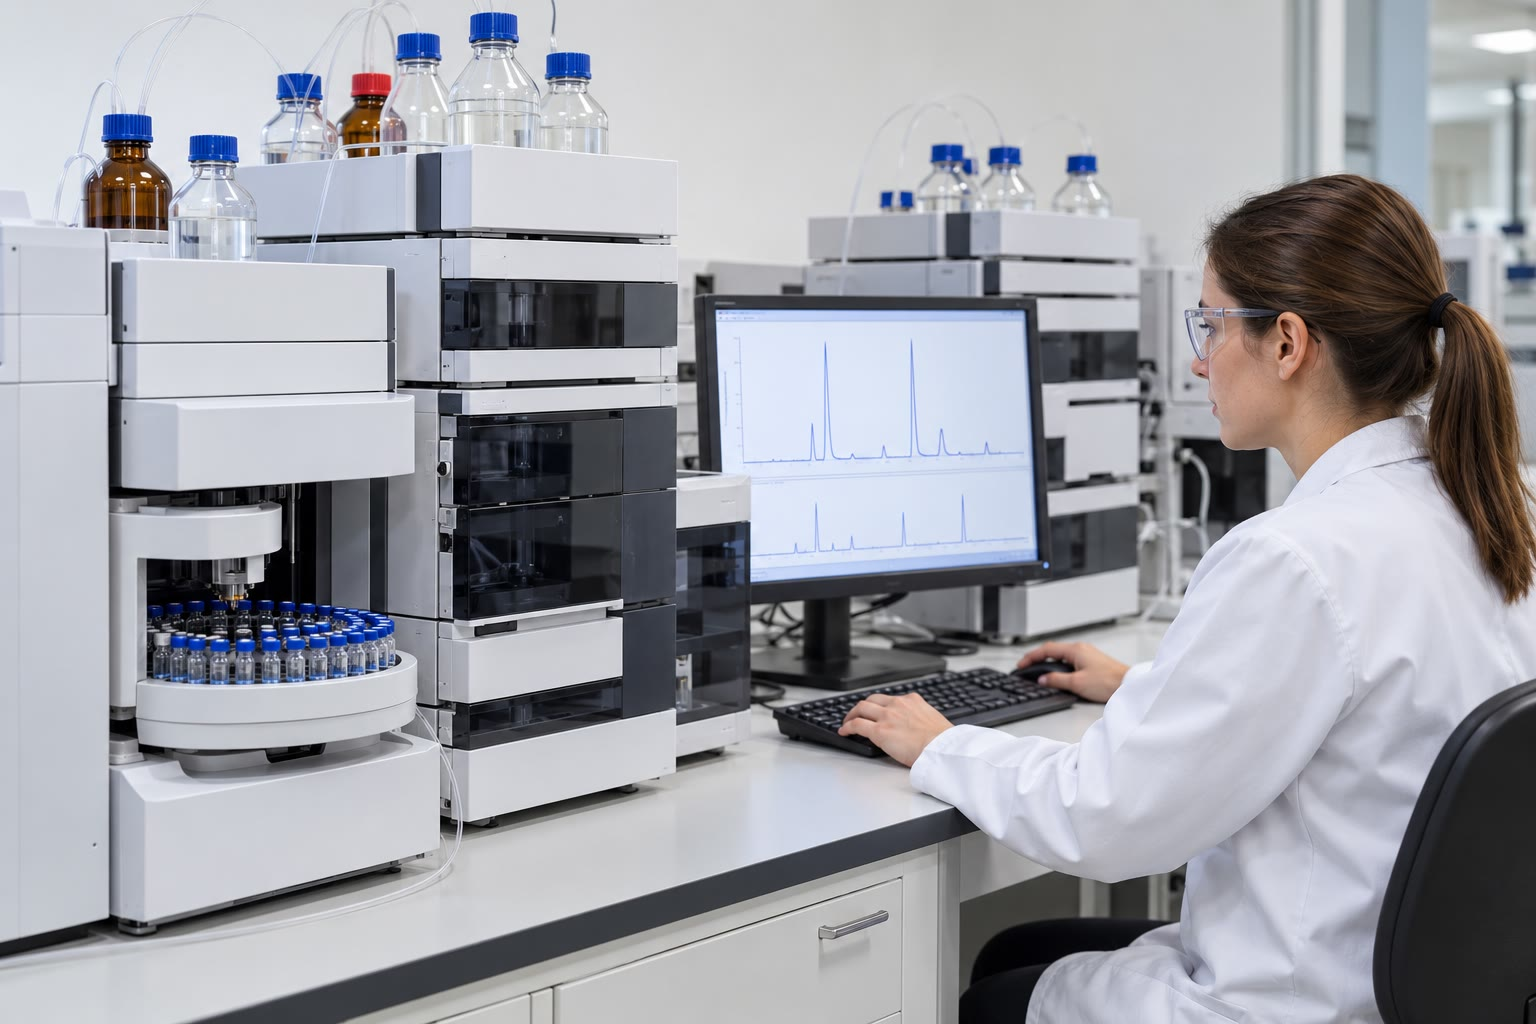
\includegraphics[width=0.58\linewidth]{images/book3/ai/b2-31-analytical-lab.jpg}

{\small एक विश्लेषणात्मक प्रयोगशाला: अपनी विलायक बोतलों के साथ द्रव वर्णलेखित्र और शीशियों की एक
स्वचालित-नमूना ट्रे; वर्णलेख स्क्रीन पर दिखते हैं (चित्रण)।}
\end{omfigure}

\begin{recall}
विद्यालय का खंड: काग़ज़ और पतली परत \omterm{def:b2:chromatography:principle}{वर्णलेखन}, वर्णलेख, निक्षालक। प्रथम वर्ष का खंड:
विभाजन गुणांक, द्रव--द्रव निष्कर्षण, पतली परत प्लेट का मंदन गुणांक $R_f$।
\Cref{ch:b2:liquid-vapour-diagrams}: आसवन स्तंभ की \omterm{def:b2:liquid-vapour-diagrams:fractional-distillation}{सैद्धांतिक प्लेट}।
\end{recall}

\section{सिद्धांत}

\begin{definition}[वर्णलेखन]\label{def:b2:chromatography:principle}
\emph{वर्णलेखन}\index{वर्णलेखन} किसी मिश्रण के घटकों को उन्हें किसी स्तंभ में या प्लेट पर स्थिर
\emph{स्थिर प्रावस्था}\index{स्थिर प्रावस्था} और उसके पास से बहने वाली गैस या द्रव, अर्थात्
\emph{गतिशील प्रावस्था}\index{गतिशील प्रावस्था}, के बीच वितरित करके पृथक करता है। गतिशील प्रावस्था के साथ घटकों को
स्तंभ से होकर बाहर ले जाना \emph{उत्क्षालन}\index{उत्क्षालन} है।
\end{definition}

कोई अणु केवल तभी चलता है जब वह \omterm{def:b2:chromatography:principle}{गतिशील प्रावस्था} में हो; जब तक \omterm{def:b2:chromatography:principle}{स्थिर प्रावस्था} उसे पकड़े रहती है, वह
प्रतीक्षा करता है। अपने मार्ग में वह दोनों प्रावस्थाओं के बीच लाखों बार अदल-बदल करता है, अतः उसकी औसत चाल
इससे निर्धारित होती है कि वह हर प्रावस्था में समय का कितना अंश बिताता है, अर्थात् उसके विभाजन साम्य से।

\begin{definition}[प्रतिधारण]\label{def:b2:chromatography:retention}
किसी यौगिक का \emph{प्रतिधारण काल}\index{प्रतिधारण काल} $t_R$ अंतःक्षेपण से उसके शिखर के
उच्चिष्ठ तक का समय है; \emph{मृत काल}\index{मृत काल} $t_M$ किसी
अप्रतिधारित यौगिक का प्रतिधारण काल है, जो कभी \omterm{def:b2:chromatography:principle}{स्थिर प्रावस्था} में प्रवेश नहीं करता। किसी स्तंभ पर किसी यौगिक का
\emph{प्रतिधारण गुणांक}\index{प्रतिधारण गुणांक k@प्रतिधारण गुणांक $k$}
$k$ यह है:
\begin{equation*}
k = \frac{t_R - t_M}{t_M}.
\end{equation*}
यह पतली परत प्लेट का $R_f$ नहीं है, जो तय की गई दूरी मापता है, यद्यपि दोनों एक ही
विभाजन का वर्णन करते हैं।
\end{definition}

\begin{proposition}[प्रतिधारण काल]\label{prop:b2:chromatography:retention-time}
यदि साम्य पर स्तंभ के किसी खंड की स्थिर और गतिशील प्रावस्थाओं में किसी यौगिक की मात्राएँ
$n_s$ और $n_m$ हों, तो यौगिक $u/(1 + n_s/n_m)$ से चलता है, जहाँ $u$ \omterm{def:b2:chromatography:principle}{गतिशील प्रावस्था} की चाल है,
और $t_R = t_M(1 + n_s/n_m)$।
\end{proposition}

\begin{proof}
कोई दिया गया अणु अपने समय का अंश $n_m/(n_s + n_m)$ \omterm{def:b2:chromatography:principle}{गतिशील प्रावस्था} में बिताता है, जहाँ वह
$u$ से चलता है, और शेष समय विराम में। उसकी औसत चाल $u\,n_m/(n_s + n_m) = u/(1 + n_s/n_m)$ है। लंबाई
$L$ का स्तंभ $t_R = (L/u)(1 + n_s/n_m)$ में पार होता है, और $L/u = t_M$।
\end{proof}

\begin{proposition}[प्रतिधारण और विभाजन]\label{prop:b2:chromatography:k-and-K}
\omterm{def:b2:chromatography:retention}{प्रतिधारण गुणांक} दोनों प्रावस्थाओं में मात्राओं का अनुपात है, $k = n_s/n_m = KV_s/V_m$, जहाँ $K$
विभाजन गुणांक है (\omterm{def:b2:chromatography:principle}{स्थिर प्रावस्था} में सांद्रता बटा \omterm{def:b2:chromatography:principle}{गतिशील
प्रावस्था} में सांद्रता) और $V_s$, $V_m$ स्तंभ में प्रावस्थाओं के आयतन हैं।
\end{proposition}

\begin{proof}
\cref{prop:b2:chromatography:retention-time} से $(t_R - t_M)/t_M = n_s/n_m$। $n_s = c_sV_s$,
$n_m = c_mV_m$ और $K = c_s/c_m$ के साथ $n_s/n_m = KV_s/V_m$।
\end{proof}

दो यौगिक तब पृथक होते हैं जब उनके विभाजन गुणांक भिन्न हों; स्तंभ की ज्यामिति ($V_s/V_m$)
सभी प्रतिधारणों को समान रूप से गुणा करती है। \omterm{def:b2:chromatography:principle}{गतिशील प्रावस्था} को बदलना, जो $K$ को बदलता है, प्रतिधारण पर रसायनज्ञ का
मुख्य उत्तोलक है।

\begin{omfigure}
\begin{tikzpicture}[x=1cm, y=1cm]
\foreach \x/\a/\b/\ha/\hb/\lab in {0/0.6/0.6/0.1/0.1/आरंभ, 2.4/1.5/2.6/0.16/0.22/बाद में, 4.8/2.4/4.4/0.2/0.3/अंत}{
  \draw[black!60] (\x-0.35,0) rectangle (\x+0.35,-5);
  \fill[omThm!55] (\x-0.33,-\b+\hb) rectangle (\x+0.33,-\b-\hb);
  \fill[omDef!55, opacity=0.85] (\x-0.33,-\a+\ha) rectangle (\x+0.33,-\a-\ha);
  \node[font=\small] at (\x,-5.4) {\lab};
}
\draw[->, thick] (-1.0,-0.3) -- (-1.0,-4.6) node[midway, left, font=\small, align=right] {गतिशील\\प्रावस्था};
\node[font=\small, align=left, anchor=west] at (5.5,-2.4) {अधिक प्रतिधारित\\(धीमा, संकरा)};
\node[font=\small, align=left, anchor=west] at (5.5,-4.4) {कम प्रतिधारित\\(तेज़)};
\draw[densely dotted] (5.15,-2.4) -- (5.5,-2.4); \draw[densely dotted] (5.15,-4.4) -- (5.5,-4.4);
\end{tikzpicture}
\par\vspace{4pt}

{\small एक साथ एक पतली पट्टी के रूप में अंतःक्षेपित दो यौगिक किसी स्तंभ में नीचे चलते हैं (तीन झलकियाँ,
व्यवस्था-रूप)। कम प्रतिधारित यौगिक (छोटा $k$) आगे दौड़ता है; चलते हुए दोनों पट्टियाँ चौड़ी होती हैं, जो
अधिक दूर गई है वह अधिक।}
\end{omfigure}

\section{शिखर की चौड़ाई और प्लेट संख्या}

कोई पट्टी पतली नहीं रहती। एक ही यौगिक के अणु कणों के बीच भिन्न पथ लेते हैं,
स्तंभ के अनुदिश विसरित होते हैं और \omterm{def:b2:chromatography:principle}{स्थिर प्रावस्था} में यादृच्छिक मात्राओं से पिछड़ जाते हैं। निकास पर
अभिलिखित शिखर लगभग मानक विचलन $\sigma_t$ (समय में) वाला एक गाउसीय वक्र होता है, और किसी दिए गए $t_R$ के लिए वह जितना
संकरा हो, स्तंभ उतना ही अच्छा।

\begin{definition}[प्लेट संख्या]\label{def:b2:chromatography:plates}
किसी यौगिक के लिए किसी स्तंभ की \emph{प्लेट संख्या}\index{प्लेट संख्या} $N = (t_R/\sigma_t)^2$ है, जहाँ
$\sigma_t$ समय में उसके शिखर का मानक विचलन है। \emph{प्लेट ऊँचाई}\index{प्लेट ऊँचाई}
$H = L/N$ है, लंबाई $L$ वाले स्तंभ के लिए।
\end{definition}

ये नाम \cref{ch:b2:liquid-vapour-diagrams} के आसवन स्तंभ से आते हैं: वर्णलेखी
स्तंभ ऐसे व्यवहार करता है मानो वह $N$ साम्य चरणों का ढेर हो, हर एक $H$ ऊँचा। यह सादृश्य गिनने का
एक तरीका है, स्तंभ का चित्र नहीं।

\begin{proposition}[शिखर से प्लेट संख्या]\label{prop:b2:chromatography:plate-number}
नति-परिवर्तन बिंदुओं पर स्पर्शरेखाओं के बीच आधार पर चौड़ाई $w$ और अर्ध-ऊँचाई पर
चौड़ाई $w_{1/2}$ के साथ,
\begin{equation*}
N = 16\left(\frac{t_R}{w}\right)^2 = 5.54\left(\frac{t_R}{w_{1/2}}\right)^2.
\end{equation*}
\end{proposition}

\begin{proof}
मानक विचलन $\sigma$ और ऊँचाई $h$ वाले गाउसीय वक्र के लिए नति-परिवर्तन बिंदु $\pm\sigma$ पर हैं,
जहाँ ऊँचाई $h\mathrm e^{-1/2}$ और ढाल $\mp h\mathrm e^{-1/2}/\sigma$ है; वहाँ की स्पर्शरेखा
$\sigma$ और आगे, $\pm2\sigma$ पर, शून्य तक पहुँचती है: $w = 4\sigma$। अर्ध-ऊँचाई वहाँ मिलती है जहाँ
$\mathrm e^{-x^2/2\sigma^2} = 1/2$, $x = \sigma\sqrt{2\ln2}$: $w_{1/2} = 2\sqrt{2\ln2}\,\sigma \approx
2.355\,\sigma$। $\sigma = w/4$ या $\sigma = w_{1/2}/2.355$ को $N = (t_R/\sigma)^2$ में रखने पर
$16$ और $2.355^2 = 5.545$ मिलते हैं, जिसे 5.54 लिखा जाता है।
\end{proof}

\begin{proposition}[वान डीम्टर समीकरण]\label{prop:b2:chromatography:van-deemter}
\omterm{def:b2:chromatography:plates}{प्लेट ऊँचाई} \omterm{def:b2:chromatography:principle}{गतिशील प्रावस्था} की रैखिक चाल $u$ पर इस प्रकार निर्भर करती है:
\begin{equation*}
H = A + \frac{B}{u} + Cu,
\end{equation*}
जहाँ $A$ भराव से होकर जाने वाले भिन्न पथों का, $B/u$ स्तंभ के अनुदिश विसरण का
(जो अणुओं के अधिक समय रुकने पर बिगड़ता है) और $Cu$ \omterm{def:b2:chromatography:principle}{स्थिर प्रावस्था} के साथ धीमे आदान-प्रदान का (जो
\omterm{def:b2:chromatography:principle}{गतिशील प्रावस्था} के तेज़ी से निकलने पर बिगड़ता है) योगदान है। $H$ $u_{\mathrm{opt}} = \sqrt{B/C}$ पर सबसे छोटा है, जहाँ $H_{\min} =
A + 2\sqrt{BC}$।
\end{proposition}

\admitted

समीकरण का रूप स्वीकृत है; उसका निम्निष्ठ नहीं। $\mathrm dH/\mathrm du = -B/u^2 + C$
$u = \sqrt{B/C}$ पर शून्य होता है, और वहाँ $B/u = Cu = \sqrt{BC}$, अतः $H_{\min} = A + 2\sqrt{BC}$; दूसरा
अवकलज $2B/u^3$ धनात्मक है, अतः यह निम्निष्ठ है। छोटे कण $A$ और $C$ को घटाते हैं: यही कारण है कि
आधुनिक द्रव \omterm{def:b2:chromatography:principle}{वर्णलेखन} कुछ माइक्रोमीटर के कण और \omterm{def:b2:chromatography:principle}{गतिशील प्रावस्था} को उनसे होकर धकेलने के लिए
उच्च दाब प्रयुक्त करता है।

\begin{omfigure}
\begin{tikzpicture}
\begin{axis}[width=0.7\linewidth, height=5.2cm, xmin=0, xmax=8, ymin=0, ymax=70,
  xlabel={रैखिक चाल $u$ (\unit{mm/s})}, ylabel={प्लेट ऊँचाई $H$ (\unit{\micro m})},
  label style={font=\small}, tick label style={font=\scriptsize},
  legend style={font=\scriptsize, at={(1.03,1)}, anchor=north west}, legend cell align=left]
\addplot[omDef, very thick] table[x=u, y=H] {figdata/out/bachelor-2-chromatogram-b.dat};
\addplot[black!50, dashed] table[x=u, y=A] {figdata/out/bachelor-2-chromatogram-b.dat};
\addplot[omThm, dashed] table[x=u, y=B] {figdata/out/bachelor-2-chromatogram-b.dat};
\addplot[omMeth, dashed] table[x=u, y=C] {figdata/out/bachelor-2-chromatogram-b.dat};
\addplot[only marks, mark=*, mark size=1.6pt] coordinates {(2,30)};
\legend{$H$, $A$, $B/u$, $Cu$}
\end{axis}
\end{tikzpicture}

{\small एक वान डीम्टर वक्र (अभ्यास के प्राचल: $A = \qty{10}{\micro m}$, $B = \qty{20}{\micro m.mm/s}$,
$C = \qty{5}{\micro m.s/mm}$)। निम्निष्ठ, $H = \qty{30}{\micro m}$, $u = \qty{2}{mm/s}$ पर, वहाँ है जहाँ
विसरण और आदान-प्रदान पद बराबर हैं।}
% figdata: bachelor-2/chromatogram.py part b
\end{omfigure}

\section{दो यौगिकों का पृथक्करण}

\begin{definition}[वरणात्मकता और विभेदन]\label{def:b2:chromatography:separation}
$k_2 > k_1$ वाले दो पड़ोसी शिखरों के लिए \emph{वरणात्मकता गुणांक}\index{वरणात्मकता गुणांक}
$\alpha = k_2/k_1$ है, और \emph{विभेदन}\index{विभेदन} यह है:
\begin{equation*}
R_s = \frac{2(t_{R2} - t_{R1})}{w_1 + w_2},
\end{equation*}
अर्थात् शिखरों के बीच की दूरी बटा उनकी माध्य आधार चौड़ाई।
\end{definition}

$R_s = 1$ पर शिखर अभी भी स्पष्ट रूप से अतिव्यापित होते हैं; $R_s = 1.5$ पर संकेत उनके बीच आधार-रेखा पर लौट आता है
(आधार-रेखा पृथक्करण), जो मात्रात्मक कार्य का सामान्य लक्ष्य है।

\begin{omfigure}
\begin{tikzpicture}
\begin{axis}[width=0.36\linewidth, height=3.6cm, xmin=-8, xmax=8, ymin=0, ymax=1.15,
  xtick=\empty, ytick=\empty, axis x line=bottom, axis y line=none, title style={font=\small},
  title={$R_s = 0.75$}]
\addplot[omDef, thick] table[x=x, y=r075] {figdata/out/bachelor-2-chromatogram-a.dat};
\end{axis}
\end{tikzpicture}\hfill\begin{tikzpicture}
\begin{axis}[width=0.36\linewidth, height=3.6cm, xmin=-8, xmax=8, ymin=0, ymax=1.15,
  xtick=\empty, ytick=\empty, axis x line=bottom, axis y line=none, title style={font=\small},
  title={$R_s = 1.0$}]
\addplot[omDef, thick] table[x=x, y=r100] {figdata/out/bachelor-2-chromatogram-a.dat};
\end{axis}
\end{tikzpicture}\hfill\begin{tikzpicture}
\begin{axis}[width=0.36\linewidth, height=3.6cm, xmin=-8, xmax=8, ymin=0, ymax=1.15,
  xtick=\empty, ytick=\empty, axis x line=bottom, axis y line=none, title style={font=\small},
  title={$R_s = 1.5$}]
\addplot[omDef, thick] table[x=x, y=r150] {figdata/out/bachelor-2-chromatogram-a.dat};
\end{axis}
\end{tikzpicture}

{\small तीन \omterm{def:b2:chromatography:separation}{विभेदनों} पर समान आकार के दो गाउसीय शिखर (मॉडल)। 0.75 पर वे मिलकर एक
द्विक बनाते हैं; 1.0 पर घाटी अभी भी ऊँचाई के एक-चौथाई पर है; 1.5 पर संकेत
आधार-रेखा पर लौट आता है।}
% figdata: bachelor-2/chromatogram.py part a
\end{omfigure}

\begin{theorem}[विभेदन समीकरण]\label{thm:b2:chromatography:resolution}
समान \omterm{def:b2:chromatography:plates}{प्लेट संख्या} $N$ वाले दो पड़ोसी शिखरों के लिए,
\begin{equation*}
R_s = \frac{\sqrt N}{4}\,\frac{\alpha - 1}{\alpha}\,\frac{k_2}{1 + k_2}.
\end{equation*}
\end{theorem}

\begin{proof}
निकट शिखरों के लिए दोनों आधार चौड़ाइयाँ लगभग समान होती हैं; दोनों को दूसरे शिखर की चौड़ाई के बराबर लीजिए,
$w = 4\sigma_t = 4t_{R2}/\sqrt N$ (\cref{def:b2:chromatography:plates})। तब $R_s = (t_{R2} -
t_{R1})/w = \sqrt N\,(t_{R2} - t_{R1})/(4t_{R2})$। $t_R = t_M(1 + k)$ के साथ
(\cref{prop:b2:chromatography:retention-time}), $t_{R2} - t_{R1} = t_M(k_2 - k_1)$ और $t_{R2} =
t_M(1 + k_2)$, अतः $R_s = (\sqrt N/4)(k_2 - k_1)/(1 + k_2)$। अंत में $k_2 - k_1 = k_2(1 - 1/\alpha) =
k_2(\alpha - 1)/\alpha$।
\end{proof}

\begin{method}[विभेदन में सुधार]\label{met:b2:chromatography:improve-resolution}
\begin{enumerate}
  \item दक्षता: $R_s \propto \sqrt N$। स्तंभ की लंबाई दुगुनी करने से $N$ और विश्लेषण समय दुगुने होते हैं
        परंतु $R_s$ केवल $\sqrt2 \approx 1.41$ से गुणा होता है; छोटे कण या इष्टतम प्रवाह दर
        नियत लंबाई पर $N$ बढ़ाते हैं।
  \item वरणात्मकता: गुणक $(\alpha - 1)/\alpha$ सबसे संवेदनशील है। \omterm{def:b2:chromatography:principle}{गतिशील प्रावस्था}
        (विलायक, pH), \omterm{def:b2:chromatography:principle}{स्थिर प्रावस्था} या, \omterm{def:b2:chromatography:techniques}{गैस वर्णलेखन} में, ताप बदलिए।
  \item प्रतिधारण: $k_2/(1+k_2)$ $k \approx 2$ तक तेज़ी से और उसके आगे धीरे बढ़ता है, जबकि समय
        $1 + k$ के अनुसार बढ़ता रहता है; $k$ को लगभग 2 और 10 के बीच रखने का लक्ष्य रखिए।
\end{enumerate}
\end{method}

\section{तकनीकें}

\begin{definition}[वर्णलेखी तकनीकें]\label{def:b2:chromatography:techniques}
\emph{गैस वर्णलेखन}\index{गैस वर्णलेखन} (GC) में \omterm{def:b2:chromatography:principle}{गतिशील प्रावस्था} एक गैस (हीलियम, हाइड्रोजन
या नाइट्रोजन) होती है और \omterm{def:b2:chromatography:principle}{स्थिर प्रावस्था} एक लंबे केशिका स्तंभ के भीतर लेपित द्रव फ़िल्म, जो
एक ओवन में रखा जाता है। \emph{उच्च-निष्पादन द्रव वर्णलेखन}\index{उच्च-निष्पादन द्रव वर्णलेखन}
(HPLC) में एक पंप द्रव \omterm{def:b2:chromatography:principle}{गतिशील प्रावस्था} को छोटे कणों से भरे एक छोटे स्तंभ से होकर
धकेलता है। \emph{उत्क्रमित प्रावस्था}\index{उत्क्रमित प्रावस्था} HPLC में \omterm{def:b2:chromatography:principle}{स्थिर प्रावस्था} अध्रुवी होती है
(लंबी ऐल्किल शृंखलाएँ धारण करने वाला सिलिका) और \omterm{def:b2:chromatography:principle}{गतिशील प्रावस्था} मेथेनॉल या
ऐसीटोनाइट्राइल के साथ जल का ध्रुवी मिश्रण। \emph{प्रवणता उत्क्षालन}\index{प्रवणता उत्क्षालन} में द्रव \omterm{def:b2:chromatography:principle}{वर्णलेखन} के दौरान
\omterm{def:b2:chromatography:principle}{गतिशील प्रावस्था} का संघटन प्रयोग के बीच बदला जाता है, ताकि प्रबलता से प्रतिधारित यौगिक तेज़ी से उत्क्षालित हों।
\end{definition}

\begin{omfigure}
\begin{tikzpicture}[x=1cm, y=1cm, box/.style={draw=black!70, rounded corners=2pt, fill=white,
  font=\small, align=center, minimum height=0.8cm, inner sep=3pt}]
\node[box] (gas) at (0,0) {वाहक\\गैस};
\node[box] (inj) at (2.2,0) {तप्त\\अंतःक्षेपक};
\draw[black!70, rounded corners=2pt, fill=omDef!8] (3.5,-1.1) rectangle (6.5,1.1);
\node[font=\small] at (5,0.85) {ओवन};
\draw[omDef, thick] (5,-0.15) circle (0.55); \draw[omDef, thick] (5,-0.15) circle (0.42);
\node[box] (det) at (8.0,0) {संसूचक};
\node[box] (data) at (10.2,0) {आँकड़ा\\तंत्र};
\draw[->, thick] (gas) -- (inj);
\draw[->, thick] (inj.east) -- (4.45,0);
\draw[->, thick] (5.55,0) -- (det.west);
\draw[->, thick] (det) -- (data);
\node[font=\footnotesize, align=center] at (5,-1.45) {केशिका स्तंभ (कुंडलित)};
\end{tikzpicture}

\medskip
\begin{tikzpicture}[x=1cm, y=1cm, box/.style={draw=black!70, rounded corners=2pt, fill=white,
  font=\small, align=center, minimum height=0.8cm, inner sep=3pt}]
\node[box] (sol) at (0,0) {विलायक\\पात्र};
\node[box] (pump) at (2.4,0) {उच्च-दाब\\पंप};
\node[box] (inj) at (4.9,0) {अंतःक्षेपक};
\draw[black!70, fill=omThm!12] (6.2,-0.18) rectangle (8.2,0.18);
\node[font=\footnotesize] at (7.2,0.45) {भरा हुआ स्तंभ};
\node[box] (uv) at (9.6,0) {UV\\सेल};
\node[box] (data) at (11.5,0) {आँकड़े};
\draw[->, thick] (sol) -- (pump); \draw[->, thick] (pump) -- (inj);
\draw[->, thick] (inj) -- (6.2,0); \draw[->, thick] (8.2,0) -- (uv); \draw[->, thick] (uv) -- (data);
\end{tikzpicture}
\par\vspace{4pt}

{\small ब्लॉक आरेख। ऊपर: एक गैस वर्णलेखित्र; नमूना अंतःक्षेपक में वाष्पित होता है, गैस द्वारा
ओवन में कुंडलित दसियों मीटर लंबे केशिका स्तंभ से होकर ले जाया जाता है, और निकास पर संसूचित होता है।
नीचे: एक द्रव वर्णलेखित्र; पंप विलायकों को मिलाता है (\omterm{def:b2:chromatography:techniques}{प्रवणता उत्क्षालन}) और उन्हें उच्च
दाब पर एक छोटे भरे स्तंभ से होकर एक UV अवशोषकता सेल तक धकेलता है।}
\end{omfigure}

दोनों के बीच चयन वाष्पशीलता से होता है। GC को ऐसे यौगिक चाहिए जो विघटित हुए बिना वाष्पित हों,
मोटे तौर पर \qty{400}{\degreeCelsius} से नीचे: विलायक, ईंधन, सुगंधें, छोटे कार्बनिक अणु। प्रयोग के दौरान
ओवन का ताप बढ़ाने से (एक ताप-रैंप) भारी यौगिक जल्दी उत्क्षालित होते हैं, जैसे HPLC में
प्रवणता करती है। HPLC हर घुलने वाली चीज़ सँभाल लेता है, जिसमें लवण, शर्कराएँ, औषधियाँ और प्रोटीन सम्मिलित हैं।
\omterm{def:b2:chromatography:techniques}{उत्क्रमित प्रावस्था} में सबसे ध्रुवी यौगिक पहले निकलते हैं और सबसे अध्रुवी अंत में; \omterm{def:b2:chromatography:principle}{गतिशील प्रावस्था} में अधिक कार्बनिक
विलायक मिलाने से हर प्रतिधारण घटता है। प्रारंभिक स्तंभ \omterm{def:b2:chromatography:principle}{वर्णलेखन}, और उसका तेज़
रूप, फ़्लैश \omterm{def:b2:chromatography:principle}{वर्णलेखन}, यही सिद्धांत बड़े पैमाने पर उत्पाद के ग्रामों के शोधन के लिए लागू करते हैं,
प्रायः ध्रुवी सिलिका पर हेक्सेन और एथिल एथेनोएट के मिश्रणों के साथ।

\section{मात्रात्मक विश्लेषण}

किसी शिखर का क्षेत्रफल संसूचक तक पहुँचे यौगिक की मात्रा के समानुपाती है, परंतु
समानुपातिकता स्थिरांक यौगिक और संसूचक पर निर्भर करता है। अंतःक्षेपित आयतन, जो
माइक्रोलीटर की कोटि के होते हैं, पूर्णतः पुनरुत्पादनीय नहीं होते। एक \omterm{def:b2:chromatography:quantitative}{आंतरिक मानक} दोनों कठिनाइयों को दूर कर देता है।

\begin{definition}[अनुक्रिया गुणांक और आंतरिक मानक]\label{def:b2:chromatography:quantitative}
\emph{आंतरिक मानक}\index{आंतरिक मानक} वह यौगिक है, जो नमूने में अनुपस्थित हो, और विश्लेषित हर विलयन में
ज्ञात मात्रा में मिलाया जाता है; उसे अन्य सभी शिखरों से विभेदित होना चाहिए और विश्लेष्य की तरह व्यवहार करना चाहिए।
आंतरिक मानक के सापेक्ष किसी विश्लेष्य का \emph{अनुक्रिया गुणांक}\index{अनुक्रिया गुणांक} $F$
इससे परिभाषित है:
\begin{equation*}
\frac{A_X}{A_{IS}} = F\,\frac{c_X}{c_{IS}},
\end{equation*}
जहाँ $A$ शिखर क्षेत्रफल हैं और $c$ अंतःक्षेपित विलयन में सांद्रताएँ।
\end{definition}

\begin{proposition}[आंतरिक-मानक मात्रांकन]\label{prop:b2:chromatography:internal-standard}
$F$, जो ज्ञात $c_X$ और $c_{IS}$ वाले अंशांकन विलयन पर मापा गया हो, \omterm{def:b2:chromatography:quantitative}{आंतरिक मानक} $c_{IS}$ पर मिलाए गए किसी नमूने के लिए,
$c_X = (A_X/A_{IS})\,c_{IS}/F$ देता है, अंतःक्षेपित आयतन चाहे जो हो।
\end{proposition}

\begin{proof}
हर क्षेत्रफल अंतःक्षेपित मात्रा के समानुपाती है: $A_X = s_X c_X v$, $A_{IS} = s_{IS} c_{IS} v$, जहाँ
संसूचक संवेदनशीलताएँ $s$ और अंतःक्षेपित आयतन $v$ है। अनुपात $A_X/A_{IS} = (s_X/s_{IS})(c_X/c_{IS})$
में अब $v$ नहीं है, और $F = s_X/s_{IS}$ विधि का एक स्थिरांक है, जो
अंशांकन विलयन पर एक बार मापा जाता है। $c_X$ के लिए हल करने पर परिणाम मिलता है।
\end{proof}

\begin{method}[आंतरिक मानक के साथ मात्रांकन]\label{met:b2:chromatography:internal-standard}
\begin{enumerate}
  \item ऐसा मानक चुनिए जो संरचना में विश्लेष्य के निकट हो, नमूने में अनुपस्थित हो, उसके निकट उत्क्षालित हो
        परंतु विभेदित हो ($R_s \ge 1.5$)।
  \item ज्ञात $c_X$ और $c_{IS}$ वाला अंशांकन विलयन अंतःक्षेपित कीजिए; क्षेत्रफल अनुपात से $F$ परिकलित कीजिए।
  \item नमूना विलयन में मानक उसी $c_{IS}$ पर मिलाइए; अंतःक्षेपित कीजिए; $A_X/A_{IS}$ पढ़िए।
  \item $c_X = (A_X/A_{IS})\,c_{IS}/F$ परिकलित कीजिए, फिर हर तनुकरण से होते हुए मूल
        नमूने तक लौटिए।
\end{enumerate}
\end{method}

बाह्य अंशांकन (केवल विश्लेष्य के मानकों की एक श्रृंखला, फिर नमूना, सभी एक ही ढंग से
अंतःक्षेपित) सरल है परंतु इस पर निर्भर करता है कि प्रयोगों के बीच अंतःक्षेपित आयतन और संसूचक स्थिर रहें।

\begin{history}[रंग-लेखन, 1906]
\begin{minipage}[t]{0.18\linewidth}
\vspace{0pt}
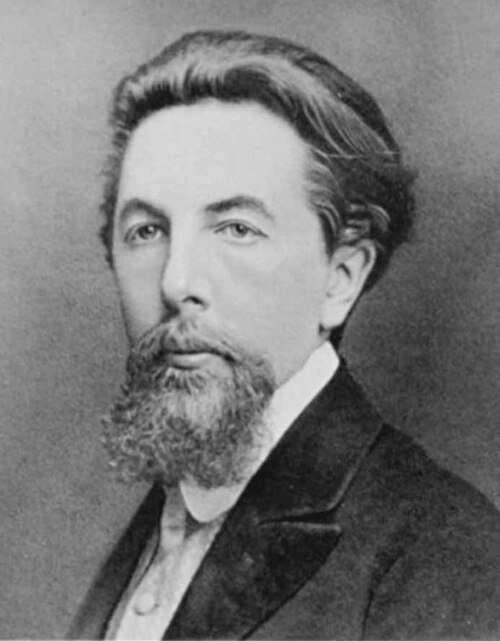
\includegraphics[width=\linewidth]{images/book3/tsvet.jpg}
\end{minipage}\hfill
\begin{minipage}[t]{0.78\linewidth}
\vspace{0pt}
वनस्पतिशास्त्री मिख़ाइल त्स्वेत ने हरी पत्तियों का एक निष्कर्ष चूर्णित खड़िया से भरी काँच की नली पर डाला
और उसे किसी विलायक से धोया: वर्णक रंगीन पट्टियों में पृथक हो गए, हरे
क्लोरोफ़िल और पीले कैरोटिनॉइड। 1906 में उन्होंने इस विधि को क्रोमैटोग्राफ़ी, ``रंग-लेखन'', नाम दिया।
एक चौथाई शताब्दी तक इसकी अधिकतर उपेक्षा हुई, जब तक कि 1930 के दशक में प्राकृतिक उत्पादों के लिए
इसे फिर नहीं अपनाया गया। (चित्र: अज्ञात लेखक, सार्वजनिक अधिकार-क्षेत्र; विकिमीडिया कॉमन्स।)
\end{minipage}
\end{history}

\begin{safety}{\ghs[5mm]{GHS02}\,\ghs[5mm]{GHS05}\,\ghs[5mm]{GHS06}\,\ghs[5mm]{GHS07}\,\ghs[5mm]{GHS08}\,\ghs[5mm]{GHS09}}
ऐसीटोनाइट्राइल और मेथेनॉल, HPLC गतिशील प्रावस्थाओं के सामान्य कार्बनिक घटक, ज्वलनशील और विषैले हैं;
स्तंभ \omterm{def:b2:chromatography:principle}{वर्णलेखन} में प्रयुक्त हेक्सेन ज्वलनशील, स्वास्थ्य के लिए ख़तरनाक और जलीय जीवों के लिए विषैला है।
विलायक अपशिष्ट एकत्र किया जाता है, कभी सिंक में नहीं बहाया जाता।
% ledger: ghs:acetonitrile, ghs:methanol, ghs:hexane
\end{safety}

\section{अभ्यास}

\begin{exercise}[$\star$]\label{exo:b2:chromatography:1}
किसी यौगिक का $t_R = \qty{5.0}{min}$ ऐसे स्तंभ पर है जिसका \omterm{def:b2:chromatography:retention}{मृत काल} \qty{1.0}{min} है। उसका
\omterm{def:b2:chromatography:retention}{प्रतिधारण गुणांक} और \omterm{def:b2:chromatography:principle}{गतिशील प्रावस्था} में बिताए गए उसके समय का अंश परिकलित कीजिए।
\end{exercise}

\begin{exercise}[$\star$]\label{exo:b2:chromatography:2}
$t_R = \qty{6.0}{min}$ पर स्थित किसी शिखर की आधार चौड़ाई \qty{0.30}{min} है। \omterm{def:b2:chromatography:plates}{प्लेट संख्या} परिकलित कीजिए।
\end{exercise}

\begin{exercise}[$\star$]\label{exo:b2:chromatography:3}
\qty{250}{mm} का एक स्तंभ किसी यौगिक के लिए $N = 10\,000$ देता है। \omterm{def:b2:chromatography:plates}{प्लेट ऊँचाई} परिकलित कीजिए।
\end{exercise}

\begin{exercise}[$\star$]\label{exo:b2:chromatography:4}
GC या HPLC? रक्त में एथेनॉल; एक प्रोटीन; किसी पेय में कैफ़ीन; पेट्रोल में बेन्ज़ीन; फलों के रस में शर्कराएँ।
\end{exercise}

\begin{exercise}[$\star\star$]\label{exo:b2:chromatography:5}
दो शिखर: $t_{R1} = \qty{4.0}{min}$, $w_1 = \qty{0.40}{min}$; $t_{R2} = \qty{4.6}{min}$, $w_2 =
\qty{0.50}{min}$। \omterm{def:b2:chromatography:separation}{विभेदन} परिकलित कीजिए। क्या वे आधार-रेखा तक पृथक हैं?
\end{exercise}

\begin{exercise}[$\star\star$]\label{exo:b2:chromatography:6}
$\alpha = 1.10$ और $k_2 = 4.0$ वाले दो यौगिकों को
$R_s = 1.5$ पर पृथक करने के लिए कितनी प्लेटें चाहिए?
\end{exercise}

\begin{exercise}[$\star\star$]\label{exo:b2:chromatography:7}
किसी स्तंभ के $A = \qty{5}{\micro m}$, $B = \qty{8}{\micro m.mm/s}$, $C = \qty{2}{\micro m.s/mm}$ हैं
(अभ्यास के आँकड़े)। इष्टतम चाल और सबसे छोटी \omterm{def:b2:chromatography:plates}{प्लेट ऊँचाई} ज्ञात कीजिए।
\end{exercise}

\begin{exercise}[$\star\star$]\label{exo:b2:chromatography:8}
जल--मेथेनॉल \omterm{def:b2:chromatography:principle}{गतिशील प्रावस्था} वाले उत्क्रमित-प्रावस्था HPLC में बेन्ज़ीन, फ़ीनॉल और टॉलूईन के \omterm{def:b2:chromatography:principle}{उत्क्षालन} के क्रम का
पूर्वानुमान कीजिए, और यह भी कि मेथेनॉल अंश बढ़ाने पर क्या होता है।
\end{exercise}

\begin{exercise}[$\star\star$]\label{exo:b2:chromatography:9}
\qty{20.0}{mg/L} पर किसी विश्लेष्य और \qty{10.0}{mg/L} पर \omterm{def:b2:chromatography:quantitative}{आंतरिक मानक} वाला एक अंशांकन विलयन
क्षेत्रफल 860 और 400 देता है। \qty{10.0}{mg/L} पर मानक मिलाया गया एक नमूना क्षेत्रफल 645 और 410 देता है।
\omterm{def:b2:chromatography:quantitative}{अनुक्रिया गुणांक} और विश्लेष्य की सांद्रता परिकलित कीजिए (अभ्यास के आँकड़े)।
\end{exercise}

\begin{exercise}[$\star\star\star$]\label{exo:b2:chromatography:10}
कोई पृथक्करण $R_s = 1.06$ देता है। वर्तमान स्तंभ के सापेक्ष कौन-सी स्तंभ लंबाई $R_s = 1.5$ देती है, और
समय में इसकी क्या क़ीमत है? और कौन-से उत्तोलक हैं?
\end{exercise}

\begin{exercise}[$\star\star\star$]\label{exo:b2:chromatography:11}
समान ऊँचाई और चौड़ाई तथा आधार चौड़ाई $w = 4\sigma$ वाले दो गाउसीय शिखरों के लिए, $R_s = 1$ और $R_s = 1.5$ पर
उनके ठीक बीच का संकेत, शिखर ऊँचाई के सापेक्ष, परिकलित कीजिए (हर उच्चिष्ठ पर दूर वाले
शिखर के योगदान की उपेक्षा कीजिए)।
\end{exercise}

\begin{exercise}[$\star\star\star$]\label{exo:b2:chromatography:12}
नियत $N$ और $\alpha$ पर \omterm{def:b2:chromatography:separation}{विभेदन} गुणक $k_2/(1+k_2)$ और आपेक्षिक विश्लेषण समय
$1 + k_2$ की तुलना कीजिए, $k_2 = 2$, 5 और 10 के लिए। आप $k$ का कौन-सा परास चुनेंगे?
\end{exercise}

\section{समस्या: एक एनर्जी ड्रिंक में कैफ़ीन}

\begin{problem}[{सप्ताहांत समस्या --- उत्क्रमित-प्रावस्था उत्क्षालन क्रम, किसी
वर्णलेख से स्तंभ का प्रदर्शन, पृथक्करण में सुधार, और आंतरिक मानक के साथ मात्रांकन}]
\label{pb:b2:chromatography:1}
अभ्यास के आँकड़े (कल्पित, कोई वास्तविक विधि नहीं)। एक एनर्जी ड्रिंक को दस गुना तनु किया जाता है (\qty{5.00}{mL} से
\qty{50.0}{mL}) और तनु विलयन में \omterm{def:b2:chromatography:quantitative}{आंतरिक मानक} के रूप में थियोफ़िलीन \qty{40.0}{mg/L} पर मिलाई जाती है।
स्तंभ: \qty{150}{mm}, \omterm{def:b2:chromatography:techniques}{उत्क्रमित प्रावस्था}; \omterm{def:b2:chromatography:principle}{गतिशील प्रावस्था} जल--मेथेनॉल; UV संसूचन।
अप्रतिधारित आधात्री (शर्कराएँ और लवण) $t_M = \qty{1.0}{min}$ पर उत्क्षालित होती है; थियोफ़िलीन
\qty{3.0}{min} पर (आधार चौड़ाई \qty{0.18}{min}); कैफ़ीन \qty{3.4}{min} पर (आधार चौड़ाई \qty{0.20}{min})।
अंशांकन: कैफ़ीन \qty{50.0}{mg/L} और थियोफ़िलीन \qty{40.0}{mg/L} क्षेत्रफल 1500 और 1000 देते हैं।
नमूना: क्षेत्रफल 970 (कैफ़ीन) और 1010 (थियोफ़िलीन)। एक डिब्बे में \qty{250}{mL} होता है।
% ledger: ghs:caffeine, ghs:methanol

\begin{center}
\begin{tikzpicture}
\begin{axis}[width=0.75\linewidth, height=4.4cm, xmin=0, xmax=5, ymin=0, ymax=1,
  xlabel={समय (min)}, ylabel={अवशोषकता (स्वेच्छ इकाई)}, label style={font=\small},
  tick label style={font=\scriptsize}, ytick=\empty]
\addplot[omDef, thick] table[x=t, y=s] {figdata/out/bachelor-2-chromatogram-c.dat};
\node[font=\scriptsize] at (axis cs:1.0,0.42) {आधात्री};
\node[font=\scriptsize] at (axis cs:2.62,0.86) {थियोफ़िलीन};
\node[font=\scriptsize] at (axis cs:3.85,0.84) {कैफ़ीन};
\end{axis}
\end{tikzpicture}
\end{center}
% figdata: bachelor-2/chromatogram.py part c

\medskip
\noindent\textbf{भाग I --- \omterm{def:b2:chromatography:techniques}{उत्क्रमित प्रावस्था}।}
\begin{enumerate}
  \item उत्क्रमित-प्रावस्था स्तंभ की स्थिर और गतिशील प्रावस्थाओं का वर्णन कीजिए।
  \item शर्कराएँ \omterm{def:b2:chromatography:retention}{मृत काल} पर क्यों उत्क्षालित होती हैं?
  \item कैफ़ीन 1,3,7-ट्राइमेथिलज़ैंथीन है, थियोफ़िलीन 1,3-डाइमेथिलज़ैंथीन। उनके \omterm{def:b2:chromatography:principle}{उत्क्षालन} के
        क्रम को समझाइए।
  \item यहाँ थियोफ़िलीन एक अच्छा \omterm{def:b2:chromatography:quantitative}{आंतरिक मानक} क्यों है?
  \item यदि मेथेनॉल अंश बढ़ाया जाए तो दोनों \omterm{def:b2:chromatography:retention}{प्रतिधारण कालों} का क्या होगा?
  \item \omterm{def:b2:chromatography:retention}{मृत काल} क्या मापता है?
\end{enumerate}

\medskip
\noindent\textbf{भाग II --- स्तंभ का प्रदर्शन।}
\begin{enumerate}[resume]
  \item थियोफ़िलीन और कैफ़ीन के \omterm{def:b2:chromatography:retention}{प्रतिधारण गुणांक} परिकलित कीजिए।
  \item \omterm{def:b2:chromatography:separation}{वरणात्मकता गुणांक} परिकलित कीजिए।
  \item कैफ़ीन और थियोफ़िलीन के लिए \omterm{def:b2:chromatography:plates}{प्लेट संख्या} परिकलित कीजिए।
  \item कैफ़ीन के लिए \omterm{def:b2:chromatography:plates}{प्लेट ऊँचाई} परिकलित कीजिए।
  \item दोनों शिखरों के बीच \omterm{def:b2:chromatography:separation}{विभेदन} परिकलित कीजिए।
  \item \omterm{def:b2:chromatography:separation}{विभेदन} समीकरण से इसकी जाँच कीजिए।
  \item क्या शिखर आधार-रेखा तक पृथक हैं?
\end{enumerate}

\medskip
\noindent\textbf{भाग III --- तेज़ या बेहतर।}
\begin{enumerate}[resume]
  \item समय बचाने के लिए स्तंभ को \qty{75}{mm} तक छोटा किया जाता है (वही भराव और प्रवाह)। \omterm{def:b2:chromatography:separation}{विभेदन} का
        क्या होता है?
  \item और विश्लेषण समय का?
  \item इसके बजाय \qty{300}{mm} का स्तंभ क्या देता, और किस क़ीमत पर?
  \item कौन-सा उत्तोलक $\alpha$ पर कार्य करता है?
  \item क्या यहाँ $k$ बढ़ाने से बहुत सहायता मिलेगी?
\end{enumerate}

\medskip
\noindent\textbf{भाग IV --- मात्रांकन।}
\begin{enumerate}[resume]
  \item थियोफ़िलीन के सापेक्ष कैफ़ीन का \omterm{def:b2:chromatography:quantitative}{अनुक्रिया गुणांक} परिकलित कीजिए।
  \item अंतःक्षेपित आयतन से कोई अंतर क्यों नहीं पड़ता?
  \item तनु विलयन में कैफ़ीन की सांद्रता परिकलित कीजिए।
  \item पेय में कैफ़ीन की सांद्रता परिकलित कीजिए।
  \item यदि कोई आधात्री यौगिक थियोफ़िलीन के साथ सह-उत्क्षालित होता तो क्या ग़लत होता?
  \item बाह्य अंशांकन के लिए इसके बजाय क्या आवश्यक होता?
  \item \qty{250}{mL} के डिब्बे में कैफ़ीन का द्रव्यमान बताइए।
\end{enumerate}
\end{problem}
